% !TEX root = ../thesis-example.tex
%
\chapter{Instances éphémères d'agencements modulaires}
\label{ch:ephemeral}

% \cleanchapterquote{Paradoxalement, la musique du futur est écrite sur du sable!}{Michel Chion}{La musique du futur a-t-elle un avenir?, 1977}

%\cleanchapterquote{Le vieux Paris n'est plus (la forme d'une ville\\
%Change plus vite, hélas ! que le coeur d'un mortel)}{Charles Baudelaire}{Le Cygne, 1861}

\cleanchapterquote{La musique (...) est trop en deça du monde et du désignable pour figurer autre chose que des épures de l'Être, son flux et son reflux, sa croissance, ses éclatements, ses tourbillons.}{Maurice Merleau-Pontry}{L'Œil et l'esprit, 1964} %\cite{merleau-ponty_loeil_1964}

\cleanchapterquote{Dufourt suggests that contemporary music highlights what was rejected in the Greek world : it rather captures the evanescent, the ephemeral, the ambivalent, the Erebus, it favors the endless metamorphosis of qualities and forms; as Nietzsche proclaimed, western music tends toward the liberation of the dyonisiac dimension and the acceptance of the inacceptable part of myths.}{Jean-Claude Risset}{Discours invité à la conférence ICMC, 2014}%\cite{risset_sound_2014} % Remettre cette citation dans le corps du texte.


%\test{blabla}
\section{Paysage des DMIs}
\label{sec:ephemerality:landscape}

%--------------------------------------------------------------
\subsection{Les origines}

\subsubsection{Pré-histoire}

Les instruments acoustiques bénéficient d'une histoire vieille de plus de 40000 ans et la finesse de leur fabrication a atteint une excellence qui fait de certains instruments de véritables pièces d'orfèvres. Les instruments numériques sont beaucoup plus récents et ne peuvent rivaliser avec ce degré de raffinement. Pour autant, il ne sont pas totalement déshérités de la tradition et du savoir-faire des instruments acoustiques et par ailleurs, le développement hautement collaboratif à l'œuvre dans le domaine de la programmation informatique fait qu'ils sont, malgré leur jeunesse, des outils extrêmement complexes et les compétences requises pour leur fabrication dépassent souvent de loin ce qu'il serait possible pour un individu seul de concevoir.

Découplage geste et énergie de production dans l'orgue.
Risset dans \cite{genevois_les_1999} ``L'orgue marque le rôle croissant de la technologie dans l'instrument de musique: il introduit le premier interrupteur, le premier clavier, et dès le XVè siècle la première synthèse additive (qui ne sera justifiée mathématiquement par Fouier qu'au XIXè siècle). L'orgue est aussi la première machine informationnelle: l'information donnée par le geste du musicien y est décuplée de l'énergie sonore''\\
Introduction de la mécanique, déport du doigté (Boehm) — révolution industrielle\\
Introduction de l'électricité (théremin, Martenot, patching de la téléphonie)\\
Introduction de l'enregistrement (phonographie, bande, Schaeffer et l'écoute réduite)\\

\subsubsection{L'arrivée du numérique}

1957 : MusicN (Music I en 1957)
1979 : Casio VL-1
1981 : IRCAM 4X
1982 : E-mu Emulator
1983 : MIDI
1983 : DX7
1985 : The Patcher
1989 : FTS/ISPW

%--------------------------------------------------------------
\subsection{Instruments augmentés}
notion d'instrument augmenté discutable (quid traverso=>Boehm ?, quid guitare électrique?) cf. \href{{sec:ephemeral:longevity_stability}}\\
smart instruments (HyVibe, MIND Music Labs)

%--------------------------------------------------------------
\subsection{Interfaces commerciales}
1ère génération MIDI : clavier, sax, guitare MIDI\\
2ème génération MPE :  LinnStrument, Seabord, SoundPlane
Synthés hybrides (Berhinger, Arturia, teenage engineering)
%--------------------------------------------------------------
\subsection{Instruments collectifs}
Laptop orchestras (Plork, Slork, L2Ork, etc.), Méta-Orchestre
Liste de langages : \url{https://github.com/toplap/awesome-livecoding#languages}

%--------------------------------------------------------------
\subsection{DIY DMIs}
Le \gls{DIY}, instruments en kit, arduino, bela, modular, ethersense, etc.

%--------------------------------------------------------------
\subsection{Live Coding}
Instrument = soft, Interface = keyboard
CucK, Tidal, TopLap, \gls{ICLC}

%--------------------------------------------------------------
\subsection{Installations sonores et instruments à la frontière}
installations sur le web (e.g. tentative d'épuisement du bruit blanc)
sonification de données
apps musicales pour smartphones

%--------------------------------------------------------------
\subsection{Musical organics}
Un mot sur la classification de Magnusson.
le terme se traduit difficilement. Organics renvoit à l'idée de l'organologie autant qu'à l'idée d'organicité, i.e. l'organisation d'un être vivant, en particulier à son organisation et sa prolifération rhizomatique.

%%%%%%%%%%%%%%%%%%%%%%%%%%%%%%%%%%%%%%%%%%%%%%%%%%%%%%%%%%%%%%%
\section{Une critique de la longévité}
\label{sec:ephemerality:critique}

\subsection{DMI will survive}

\noindent La longévité des \glspl{DMI} est une question complexe qui a été soulevée à plusieurs reprises dans la littérature des \gls{NIME} (et d'autres domaines connexes) et a fait l'objet d'un débat croissant au cours de la dernière décennie \cite{baguyos_contemporary_2014} \cite{morreale_design_2017} \cite{bonardi_preservation_2008}. Les auteurs qui se sont intéressés à cette question ont identifié un certain nombre de causes de cette situation, qu'elles soient techniques, méthodologiques ou sociologiques et ont apporté réflexions et propositions pour y remédier, telles que de nouveaux environnements pour concevoir et évaluer les instruments \cite{jorda_digital_2004} \cite{morreale_design_2017}, une meilleure documentation, de nouvelles méthodes pédagogiques et la création de communautés ainsi qu'un travail visant à établir une notation musicale et un répertoire pour ces nouveaux instruments \cite{mamedes_composing_2014}\cite{mays_notation_2014}. Cependant, dans la majorité de ces articles, le manque de longévité des \glspl{DMI} est essentiellement considéré comme un défaut, ou du moins un problème à résoudre.\\
\indent Dès 1975, des compositeurs de musique électroacoustique au \gls{GRM} réfléchissaient aux questions de préservation soulevées par une musique \iquote{écrite sur du sable}\footnote{Michel Chion utilise cette formule dans \cite{chion_musique_1977}, en faisant référence aux particules ferro-magnétiques des bandes audio, vouées à une dégradation prochaine} : certains compositeurs disaient qu'ils s'en moquaient et faisaient leur musique pour le présent, tandis que d'autres voyaient dans l'ère numérique naissante la possibilité de préserver leurs œuvres dans le futur. Comme nous le savons aujourd'hui, troquer le sable contre le silicium (ou le nuage, maintenant) n'a pas totalement résolu le problème.\\
\indent Les \glspl{DMI} ayant largement intégré la partie compositionnelle des œuvres musicales, parfois même confondue avec l'instrument, le désir de préserver les œuvres musicales s'est trouvé partiellement transposé dans la question de la conservation des instruments et des outils utilisés pour leur production. Mais quelles sont les raisons de cette quête de longévité ? Et qu’est ce qui légitime à ce point la longévité d’un instrument pour qu’elle soit d’emblée vue comme une qualité ? 

\indent Le désir de longévité est lié ontologiquement à une réaction profondément enracinée dans notre condition de simples mortels, qui consiste à chercher un moyen d'assurer notre survie, notamment par la transmission des connaissances et la création de traditions. Le paléoanthroplogue André Leroi-Gourhan a analysé le phénomène des traditions comme un moyen d'extérioriser et de transmettre notre mémoire à travers la création de systèmes techniques et de ``chaînes opératoires'' \cite{leroi-gourhan_geste_1964}. Plus récemment, Bernard Stiegler s'est appuyé sur cette idée (todo : faut il citer aussi Simondon et Auroux ici?) pour définir le concept de ``grammatisation'', comme processus par lequel le continuum temporel des comportements humains est transformé en un spatial discret, ce qui permet de les intégrer dans des outils \cite{stiegler_for_2010}.\\
\indent Les humains ont ainsi développé des méthodes et des outils tels que la psalmodie de textes (surtout religieux), ou l'écriture comme moyens à la fois d'enregistrer des informations pour un usage ultérieur et de transmettre des connaissances à ceux qui y survivent. L'écriture a partiellement libéré l'homme du besoin de tradition orale en transférant ces connaissances sur un support physique, ce qui lui a également permis de capitaliser et de spéculer sur ses connaissances.\\
\indent Ainsi, la notion de longévité traverse le champ des arts et des sciences, aux frontières desquels se trouvent les instruments de musique. Dans l'histoire de l'art, il reste principalement les œuvres durables, ``gravées dans la marbre'' dont sont faites les sculptures. De même, la science aspire à trouver des lois durables pour décrire le monde observable, et les formuler dans le langage pérenne des mathématiques. Mais si la longévité évidente d'une œuvre constitue souvent un atout pour sa propre légitimation, lorsqu'il s'agit d'un instrument numérique, et plus encore lorsqu'il est conçu comme un moyen interactif de créer une expérience musicale par essence éphémère, la question ne semble pas pouvoir se régler dans les mêmes termes.\\

	
\subsection{Longevité, adoption, succès}
\noindent Deux aspects semblent être souvent confondus : la longévité d'un instrument d'une part et son ``succès'' d'autre part. De plus, la notion de succès, éminemment sujette à la perspective adoptée, semble être souvent considérée comme le taux d'adoption par une communauté d'instrumentistes, au delà des aspects financier d'un succès commercial.\\
\indent Ces trois aspects, longévité, succès et adoption, sont cependant relativement différents, en partie indépendants et même parfois contradictoires. Il existe des exemples notoires de ce décalage: The Hands de Michel Waisvisz \cite{torre_hands:_2016} (Figure \ref{fig:ephemeral:Waisvisz_TheHands}) ou encore le Méta-Instrument de Serge De Laubier \cite{couprie_meta-instrument:_2018} (Figure \ref{fig:ephemeral:DeLaubier_MI4}) sont deux instruments ayant eu une longévité remarquable\footnote{Plus de 20 ans pour The Hands —jusqu'au décès de Michel Waisvisz, et plus de 30 ans pour le Méta-Instrument dont l'actuelle 4ème version a été finalisée en 2019.}, soutenue par une pratique régulière de leur inventeurs, sans toutefois avoir été adopté par une large communauté d'instrumentistes. Inversement, l'éphémérité d'un outil ne mène pas systématiquement à une absence de popularité \footnote{Considérons ici tous les gadgets éphémères qui, sous l'influence d'une mode et/ou d'une puissante campagne publicitaire, envahissent le marché, ou encore tous les appareils qui deviennent obsolètes lorsqu'un nouvel appareil les remplace, tel que le smartphone qui, outre le remplacement de nos anciens téléphones, a également balayé d'un coup les lecteurs mp3, les GPS, les consoles de jeux portables, les lampes de poche, les montres, etc.} et encore moins à un manque d'intérêt musical pour les performances réalisées avec ces instruments.

%------------------ Figure : Waisvisz — De Laubier ---------------------
\begin{figure}[!htbp]
	\makebox[\linewidth][c]{%
		\begin{subfigure}[b]{.5\textwidth}
			\centering
			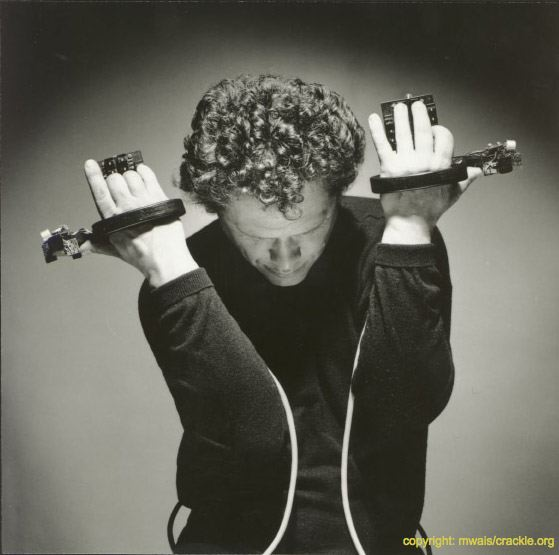
\includegraphics[width=.95\textwidth]{gfx/02_ephemeral/Waisvisz_TheHands.jpg}
			\caption{Michel Waisvisz, The Hands v2\\ photographie: Carla van Thijn}
			\label{fig:ephemeral:Waisvisz_TheHands}
		\end{subfigure}%
		\begin{subfigure}[b]{.5\textwidth}
			\centering
			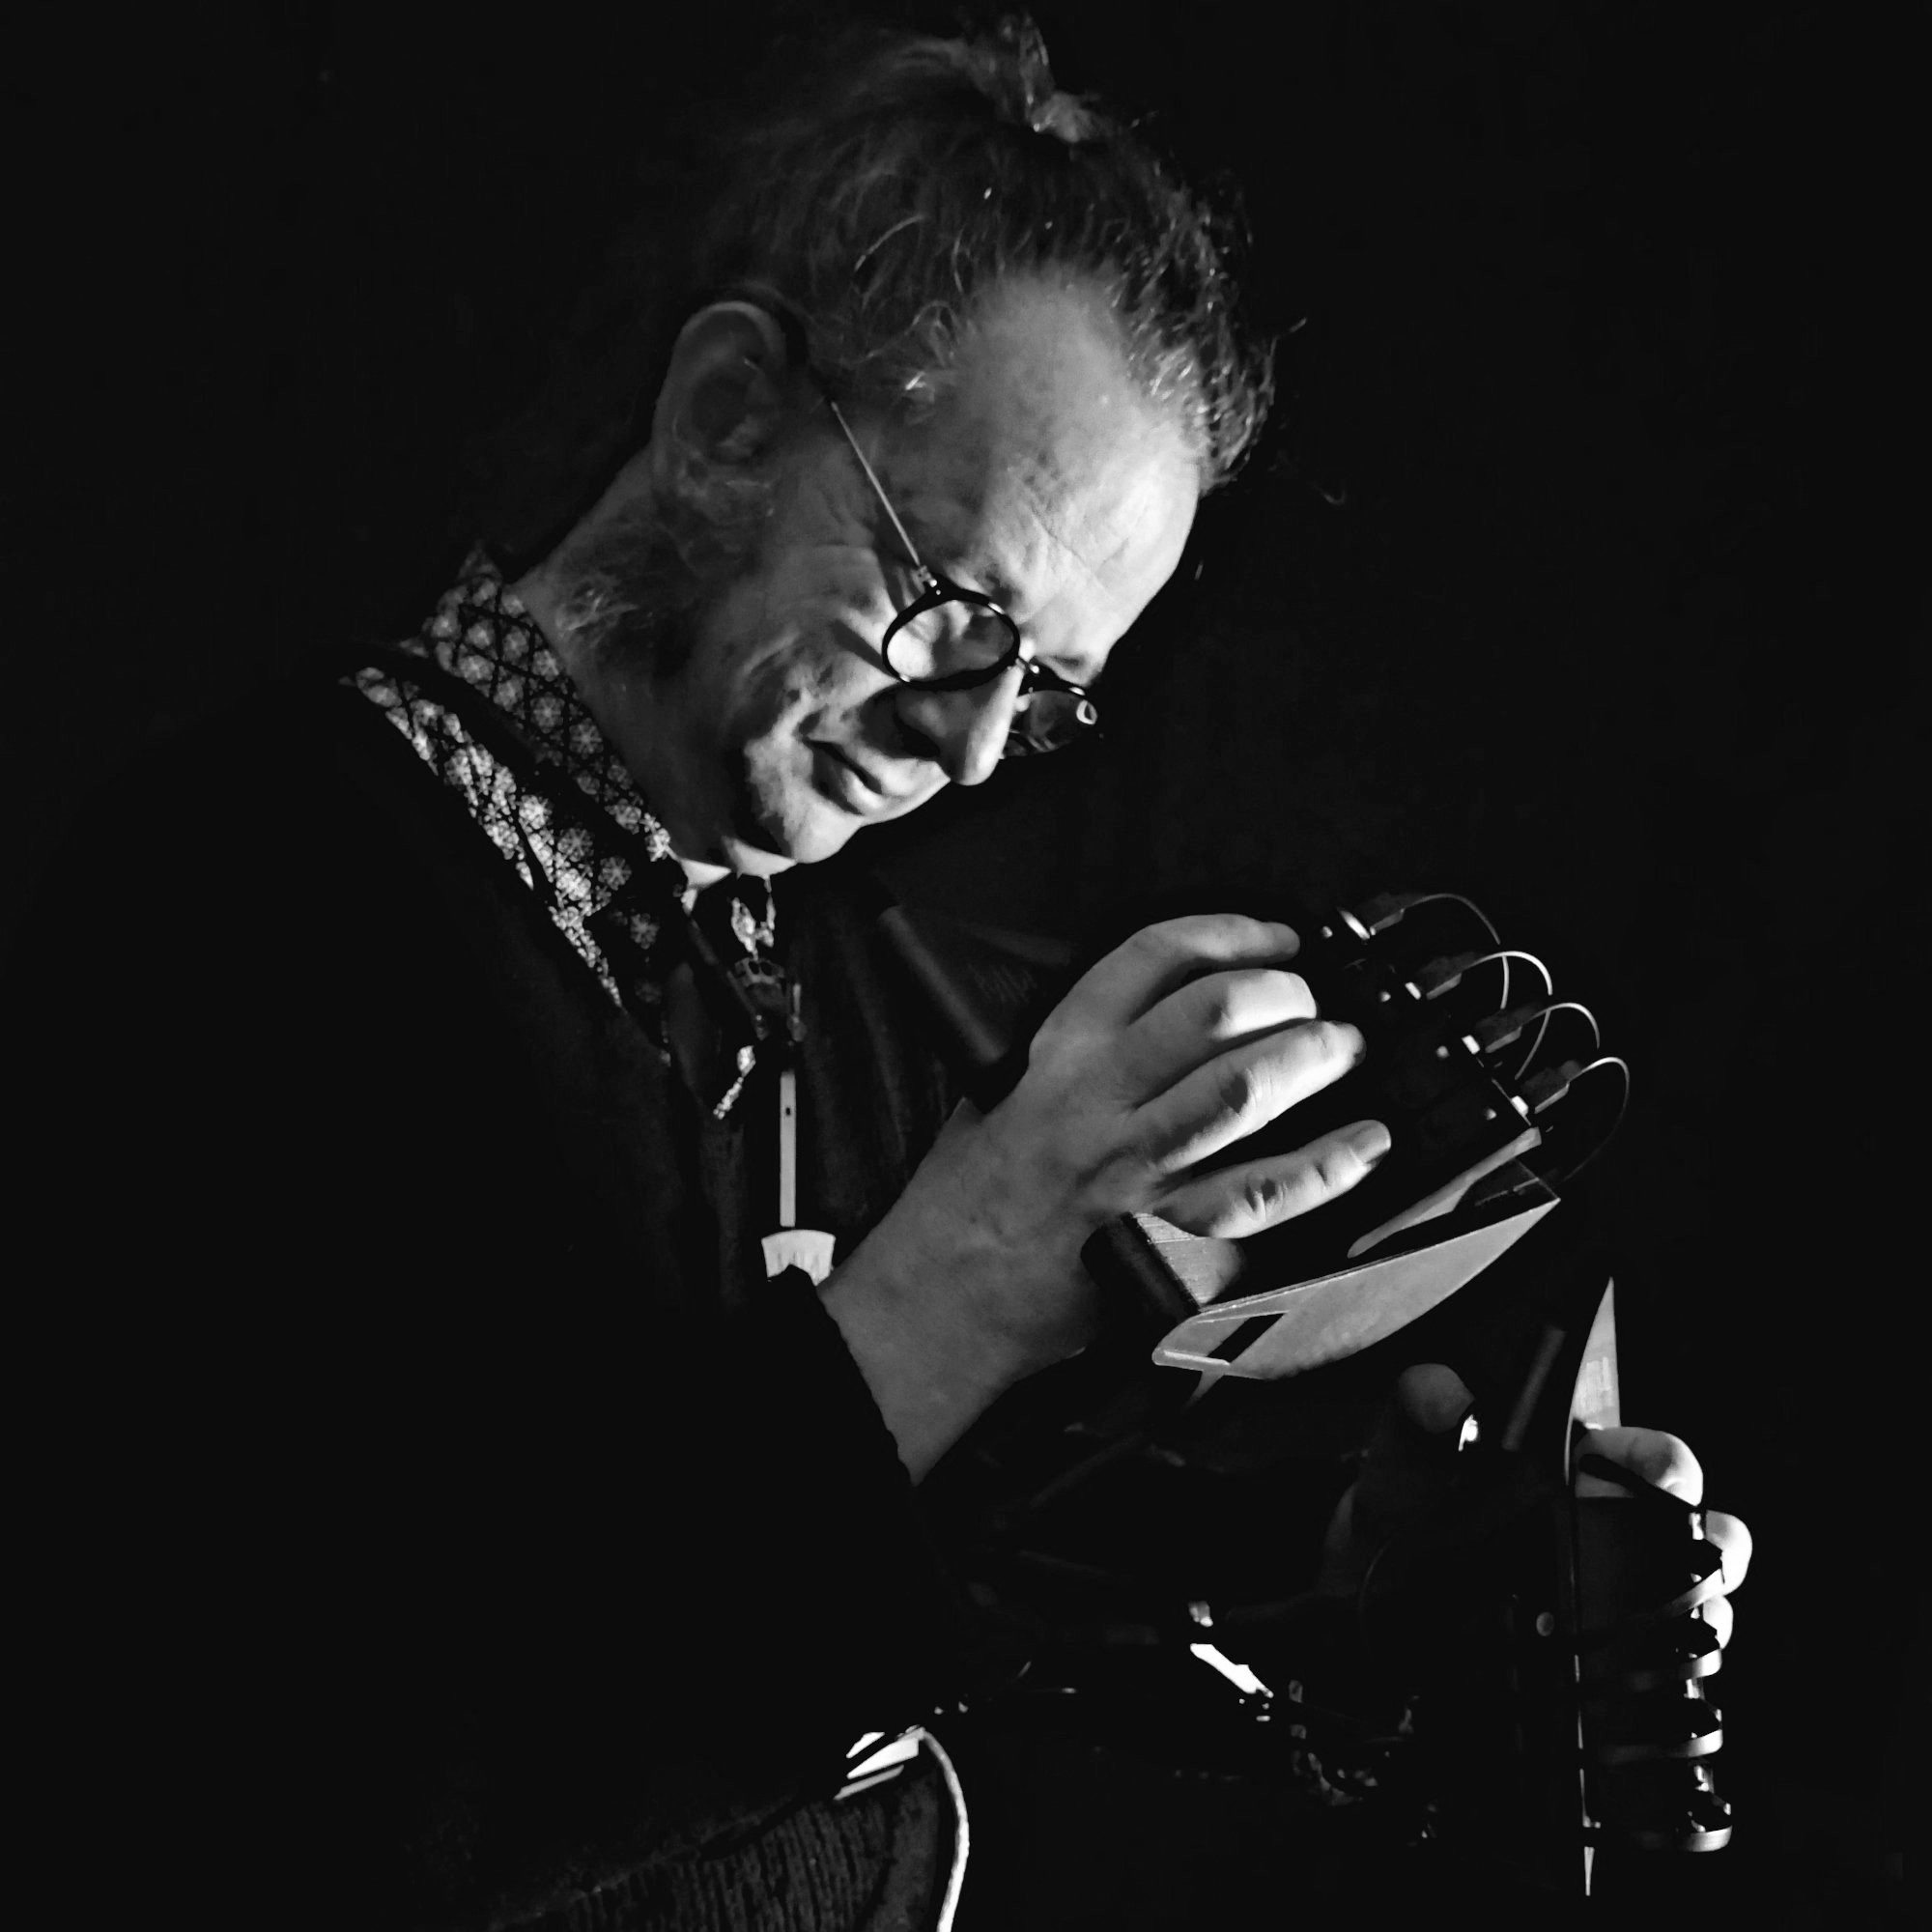
\includegraphics[width=.95\textwidth]{gfx/02_ephemeral/DeLaubier-MI4.jpg}
			\caption{Serge de Laubier, Méta-Instrument 4\\ photographie: Puce Muse}
			\label{fig:ephemeral:DeLaubier_MI4}
		\end{subfigure}%
	}
	\caption{The Hands v2 et le Méta-Instrument 4: durabilité n'est pas synonyme d'adoption}
\end{figure}

\indent La notion de succès dépend ainsi de la perspective adoptée, selon qu'elle soit celle des luthiers qui créent des instruments pour d'autres ou de ceux qui créent des instruments pour eux-mêmes. Dans ce dernier cas, l'adaptation de l'instrument aux besoins ou à l'esthétique propres de l'instrumentiste peut s'avérer telle qu'il soit difficile pour les autres de l'adopter.\\
\indent Egalement, les évolutions techniques ainsi que les modes peuvent amener à la réapparition d'instruments tombés dans l'oubli. On appréciera ici la perspicacité de François-Alexandre Garsault, cité par Malou Haine dans \cite{haine_les_2018}, qui dans sa D``ivision des instruments selon leurs différentes utilisations'' (1761) classait une série d'instruments, dont la harpe et la ``guitare'' (sic), dans la catégorie des \iquote{Instruments hors d'usage, mais qui peuvent revenir.}


\subsection{Longevité versus stabilité}
\label{sec:ephemeral:longevity_stability}
La question de la durabilité d'un instrument soulève implicitement la question de sa stabilité historique. Ainsi, l'histoire organologique des instruments de musique européens révèle de nombreux facteurs qui conduisent à l'apparition, à l'évolution ou à la disparition des instruments de musique. A cet égard, les nombreuses innovations technologiques de la révolution industrielle s'avèrent intéressantes car cette période bien documentée illustre les débuts des grandes révolutions qui allaient se produire au XXe siècle, tout en soulevant la question même de la stabilité de la forme des instruments. Ainsi, lorsque le traverso fut équipée du système de clétage inventé par Théobald Boehm en 1832 et devint une flûte traversière, s'agissait-il d'un nouvel instrument ? À quel moment décidons-nous qu'un instrument qui subit des changements n'est plus le même ?

\subsection{Éphémérité dans le contexte musical}
\label{sec:ephemeral:ephemerality_in_musical_context}

\subsubsection{Impermanence du phénomène sonore}
\noindent Rappelons tout d'abord une évidence : la musique elle-même est intrinsèquement intangible, évanescente et nécessite une énergie entretenue pour exister : le phénomène sonore est en éphémèrité permanente. La musique, dans sa forme sensible, n'existe que pendant le temps de son performance. Bien que les instruments utilisés pour la produire puissent être durables, leur convocation et le son lui-même sont toujours temporaires\footnote{à tel point que les pièces qui mettent au défi cette éphémérité, telles que les Vexations d'Erik Satie ou encore Organ²/ASLSP de John Cage sont des exceptions notoires.}.

\subsubsection{De la performance}

\noindent Même lorsqu'elle est notée sur une partition, la musique en tant que qu'art vivant est en constante réinterprétation. Cette interprétation permet de transformer une partition notée sous forme symbolique en une expression sensible sujette à variations. On peut objecter que cette interprétation n'existe que lorsque la musique est notée de manière symbolique, laissant aux interprètes la possibilité de la jouer à leur façon dans le contexte de l'interprétation. Mais est-ce toujours le cas lorsque la musique est `intégralement notée' jusqu'au son lui-même, comme c'est le cas sur un disque audio ? Cela signifie-t-il que l'interprétation disparaît ? Les performances de spatialisation en direct de la musique électroacoustique par des musiciens professionnels ou les différentes pratiques de remixes que l'on retrouve dans le hip-hop tendent à prouver le contraire. Toute performance musicale, même la simple écoute d'un disque, convoque inévitablement un nouveau contexte d'écoute, car elle se produit nécessairement dans un moment présent unique. Entre le son enregistré et son écoute, on retrouve la même \textit{différance}\footnote{La \textit{Différance} est un concept proposé par Derrida \cite{derrida_lecriture_2014} pour désigner à la fois l'ajournement (le fait de différer) et la différenciation qui se créé entre un texte et sa signification.} qu'entre une partition et ses interprétations.

\subsubsection{Une esthétique musicale mûe par le mouvement}

\noindent Par ailleurs, la musique contemporaine occidentale poursuit une quête de la nouveauté et de territoires sonores inexplorés, comme le soulignait Jean-Claude Risset dans son discours à Athènes en 2014 \cite{risset_sound_2014}: \iquote{Dufourt suggests that contemporary music highlights what was rejected in the Greek world : it rather captures the evanescent, the ephemeral, the ambivalent, the Erebus, it favors the endless metamorphosis of qualities and forms; as Nietzsche proclaimed, western music tends toward the liberation of the dyonisiac dimension and the acceptance of the inacceptable part of myths.}

\subsubsection{Partitions dynamiques, ouvertes, ad-hoc}

\noindent Les partitions musicales sont en partie intégrées dans les \glspl{DMI}, pour lesquels Norbert Schnell et Marc Battier ont proposé le terme `d'instruments composés' dans \cite{schnell_introducing_2002}\footnote{L'idée d'instruments composés est toutefois plus ancienne, voir Harry Partch ou Gordon Mumma (1967) : \iquote{I consider that my designing and building circuits is really ‘composing’ y my ‘instruments’ are inseparable from the compositions themselves.}\cite{mumma_creative_1967}}. La partition elle-même a fait l'objet d'une reconfiguration plus ouverte depuis le milieu du XXe siècle et les compositeurs ont progressivement intégré les possibilités algorithmiques dans leurs processus de création : des systèmes dynamiques et interactifs mettent en mouvement la stabilité des figures de notes. Plusieurs compositeurs\footnote{Parmi ceux qui ont écrit et analysé des partitions dynamiques, voir les œuvres de Hajdu \cite{hajdu_disposable_2016}, Bhagwati \cite{bhagwati_vexations_2017} ou Freeman \cite{freeman_extreme_2008}} questionnent ainsi la stabilité de la partition en utilisant l'ordinateur pour créer des instances \textit{ad hoc}, soit à l'aide d'algorithmes génératifs, soit en introduisant des parties improvisées dans des formes hybrides pour lesquelles Richard Dudas propose le terme de ``comprovisation'' \cite{dudas_comprovisation:_2010}. En est-il ainsi, que la technologie numérique offre ce support idéal qui permettrait à la fois la préservation des œuvres musicales en même temps que leur mutation ?

\subsubsection{Obsolescence de la technologie}

\noindent Les matériaux utilisés pour les instruments acoustiques semblent vieillir relativement bien. Le matériel électronique vieillit mal en comparaison et le cuivre de ses circuits est plus fragile que celui des trompettes, saxophones et autres cuivres. Par ailleurs, la miniaturisation extrême des microprocesseurs les rend souvent impossibles à réparer ; ils sont souvent remplacés par de nouvelles versions possiblement incompatibles. Le code informatique, dans sa forme compilée, est tout aussi cryptique que le microprocesseur : un bloc illisible qui incarne le paradoxe de la notation informatisée par rapport au papier traditionnel - ``nous écrivons des choses que nous ne pouvons plus relire''\footnote{Kevin Slavin dans la conférence ``Comment les algorithmes façonnent notre monde'', \url{https://www.ted.com/talks/kevin_slavin_how_algorithms_shape_our_world}}. Et quand le système d'exploitation sera mis à jour, il y a des chances qu'il ne pourra plus les lire non plus.\\
\indent Dans un article où il compare les différences ontologiques entre \textit{hardware} et \textit{software}, Nicolas Collins \cite{collins_semiconducting_2013} résume leur relation au temps avec la formule : \iquote{hardware is yesterday, software is now}, ce qui pourrait se traduire par le fait que le logiciel est en permanente mise à jour tandis que le hardware est toujours dépassé. Ni l'un ni l'autre ne semble être en mesure d'offrir une continuité fiable entre le passé et l'avenir.

	
\subsubsection{Economie de la nouveauté}

\noindent A l'obsolescence de la technologie, s'ajoutent les effets de la société de consommation. Depuis plus d'un siècle, l'industrie fait de plus en plus la promotion d'un paradigme jetable en encourageant les consommateurs à \iquote{acheter pour le style, pas seulement pour les améliorations technologiques} \cite{slade_made_2006} et en organisant une obsolescence programmée.\\
\indent Ce modèle économique a également affecté celui des arts du spectacle, qui promeut la création bien plus que la reprise d'un spectacle à tel point que, comme le rappelle Georg Hajdu dans \cite{hajdu_disposable_2016} : \iquote{Les pièces connaissent rarement plus qu'une seule représentation}. De même, les résidences d'artistes sont plus souvent destinées à de nouvelles créations davantage qu'à la poursuite d'œuvres antérieures.\\
\indent Cette économie de l'obsolescence (planifiée ou non) ne favorise pas l'attachement à un instrument et, en ce qui concerne les contrôleurs MIDI commerciaux, le plastique bon marché dont ils sont le plus souvent faits dégrade la valeur qui peut être attribuée à un instrument acoustique traditionnel. L'attachement et l'engagement avec les instruments virtuels sont également remis en question par leur nature immatérielle. La plupart des logiciels commerciaux s'orientent maintenant vers une économie de basée sur l'abonnement plutôt que sur l'achat, puisque l'achat ne garantit plus ni la durabilité ni la propriété de l'objet.

	
\subsubsection{L'instrument comme compromis instable}

\noindent L'instrument de musique est aussi, comme le souligne Bernard Sève dans \cite{seve_instrument_2013} : \iquote{un compromis instable entre des qualités non-convergentes}. Pour les instruments acoustiques, ce compromis entre ergonomie gestuelle et performance acoustique, imposé par la physicalité des matériaux, est généralement fixé dans un assemblage ajusté et collé. Ce montage agit comme un facteur de stabilisation par rapport à un environnement numérique dans lequel l'absence de contrainte physique laisse l'instrument à cœur ouvert, prêt à être modifié à tout instant.\\
\indent Bill Buxton soulignait la différence entre les spécifications standard, militaires et artistiques pour souligner l'exigence plus élevée de cette dernière \cite{buxton_artists_1997}. Le design des objets d'art exige une grande finesse, en effet. Accorder les qualités sonores et ergodynamiques\footnote{Thor Magnusson a proposé ce terme dans \cite{magnusson_ergodynamics_2019} pour nommer le \iquote{pouvoir et la profondeur expressive d'un instrument}} d'un instrument de musique s'apparente à la quête d'un \textit{inframince}\footnote{Marcel Duchamp \cite{duchamp_notes_2008} a inventé le terme inframince dans une série d'exemples décrivant une différence si petite qu'elle ne peut être qu'imaginée} pour lequel il n'existe pas de spécifications convenues. Mais une autre particularité des technologies utilisées pour les performances live est qu'elles sont \iquote{dévolues à une expérience, pas à une bande-son, inutiles pour la relecture, la sauvegarde, l'échange ou la duplication}, comme le note Nicolas Collins dans \cite{collins_semiconducting_2013}.\\
\indent Ainsi, la pérennité de l'instrument en dehors de la durée même de la performance n'est pas un critère essentiel et il n'est pas rare que les musiciens numériques\footnote{Andrew Hugill définit un \textit{musicien numérique} dans \cite{hugill_digital_2019} comme \iquote{quelqu'un qui a saisi les possibilités ouvertes par les nouvelles technologies, en particulier le potentiel de l'ordinateur pour explorer, stocker, manipuler et traiter le son, ainsi que le développement de nombreux autres outils et dispositifs numériques qui permettent l'invention et la découverte musicale} soulignant le fait qu'ils sont \iquote{non pas définis par leur seule utilisation de la technologie}, mais ont aussi \iquote{une certaine curiosité, un questionnement et un engagement critique sur ce terrain.}} de modifier leur instrument quelques minutes avant le début d'un concert, juste pour les besoins du moment présent.

	
\subsubsection{Esthétique du dysfonctionnement}

\noindent En effet, le risque de dysfonctionnement n'est pas rédhibitoire à de nombreuses performances musicales. Les bugs et artefacts causés par les dysfonctionnements s'avèrent être des sources fertiles de matériaux musicaux et la subversion du fonctionnement cryptique des processeurs en révèle un aspect invisible, faisant ressurgir la nature même du matériau électronique, au-delà de l'objectif pour lequel ils ont été conçus\footnote{Parmi les exemples significatifs, les travaux de Yasuano Tone pour ``Wounded CD'', ceux de Nicolas Collins sur circuits électroniques morts ou encore la sonification de données brutes par Carsten Nicolai illustrent clairement cette approche}. David Zicarelli, cité par Cascone dans \cite{cascone_aesthetics_2000}, le résume en ces termes : \iquote{Je remarque simplement que dans la plupart des concerts pointus, l'échec a tendance à être beaucoup plus intéressant pour le public que le succès.}

\subsubsection{Plus besoin de tradition?}

\noindent L’apparition de la notation musicale ne rend plus nécessaire la performance à de seules fins de transmission, l’enregistrement audio ne rend plus nécessaire la performance à de seules fins d’écoute, l’existence de banques de sons ne rend plus nécessaire l’apprentissage d’un instrument particulier pour produire le son de cet instrument\footnote{Voir par example, le rendu du Sacre du Printemps d'Igor Stravinsky par Jay Bacal avec la Vienna Sound Library (VSL): \url{https://youtu.be/PB3njyDW8SY.}}, et maintenant l’intelligence artificielle rend superflu l'acte même de composition pour que de la musique soit composée\footnote{Voir par exemple les productions du projet FlowMachines par François Pachet et al. in \cite{hadjeres_deepbach:_2016}: “Daddy's car” (\url{https://youtu.be/LSHZ_b05W7o}) ou “DeepBach” (\url{https://youtu.be/QiBM7-5hA6o}).}.\\
\indent En 1964, André Leroi-Gourhan, qui voyait dans la machine informatique la possibilité sans précédent d'externaliser la mémoire, se demandait alors ce qui adviendrait si les machines devenaient capables de \iquote{d’écrire des pièces de théâtre parfaites, peignait des tableaux inimitables}\cite{leroi-gourhan_geste_1964}. En 1992, John Cage semblait lui répondre de façon radicale : \iquote{Nous n'avons pas besoin d'avoir des traditions si nous nous libérons de la mémoire.} \cite{sebestik_ecoute_1992}. \\
\indent Cependant, s'il est possible d'évoluer, comme le décrit la philosophe Christine Buci-Glucksmann dans \cite{buci-glucksmann_esthetique_2003}, d'une culture de l'objet à une culture des flux, elle remarque que dans un pays comme le Japon qui valorise positivement l'impermanence, l'éphémère a une place centrale tout en étant profondément ancré dans la tradition.\\
\indent La résolution de cet antagonisme apparent entre la position de Cage et celle de Buci-Glucksmann semble se situer dans le déplacement des objets (ou des flux, en l'occurence) soutenus par la tradition, dans la reformulation des motivations de la pérennité et de l'éphémèrité.

\section{Articulation du pérenne et de l'éphémère}

\subsection{Les DMI comme agencements instables et sauvages}

\noindent Le terme même de \gls{DMI}, qui a progressivement envahi la littérature des \gls{NIME}, pourrait nous laisser penser qu'il s'agit d'une catégorie bien définie alors qu'il s'agit en fait d'un méli-mélo d'objets qui n'ont de commun que leur utilisation de la computation numérique. Le biais qui en résulte dans l'évaluation de l'incapacité des \glspl{DMI} à atteindre une maturité provient du fait qu'un instrument de musique est encore souvent considéré comme un tout cohérent, devant faire preuve de longévité, à l’image des instruments acoustiques pris comme modèles.\\
\indent Pourtant, la modularité induite par l'électronique et la technologie numérique a ``atomisé'' l'intégrité de l'instrument. Cette atomisation peut être entendue à la fois dans le sens de ``détruit'' mais aussi dans le sens de ``fragmenté en éléments atomiques''. Sur scène, on constate en outre que les \glspl{DMI} s'apparentent souvent à des assemblages prototypiques fragiles\footnote{Pour une réflexion poursuivant à dessein la fragilité —et la destructibilité— des \glspl{DMI}, voir aussi \cite{haddad_fragile_2017}} (cf. Figure \ref{fig:ephemeral:Gordeff}), pleins de câbles (physiques ou virtuels) prêts à être intervertis quelques minutes avant le concert, ou même pendant celui-ci. Pourquoi dans ce cas les envisager comme des monolithes durables plutôt que comme les agencements\footnote{Adoptant ici le concept de Deleuze et Guattari proposé dans \cite{deleuze_mille_1980}; voir aussi ``musical instruments as assemblage'' de Paul Theberge dans \cite{bovermann_musical_2017}.} éphémères qu’ils sont le plus souvent?\\
\todo{évoquer la notion de behavioural objects de \cite{bown_understanding_2009}}
\indent De ce point de vue, le format académique d'une conférence telle que \gls{NIME} rend difficile la présentation des \gls{DMI} dans leur forme chaotique et leur sélection est biaisée par le fait que leurs auteurs appartiennent souvent au monde académique. Cela favorise la démonstration de critères techniques dûment réfléchis plutôt que la présentation d'un fatras de circuits et d'algorithmes connectés empiriquement et dont on ne comprend rien au fonctionnement, sinon que le musicien qui en joue fait des merveilles.\\
\indent En se confrontant à un agencement instrumental éphémère, l'instrumentiste, tout virtuose qu'il soit, se retrouve nécessairement en tension avec un instrument ``sauvage'' qu'il faut apprivoiser. Cela demande une attention gestuelle et auditive intense et la recherche de résonance avec l'instrument. (Sinon, autant composer tranquillement chez soi et fournir à l’auditeur un support sur lequel il n’aura qu’à appuyer sur la touche \textit{play}). Peut-être davantage que la longévité, on pourra y voir un critère de lutherie intéressant : la possibilité que l'instrument dérape et devienne hors de contrôle.

%-------------------------- Figure : Gordeff ----------------------------------
\begin{figure}[!htbp]
	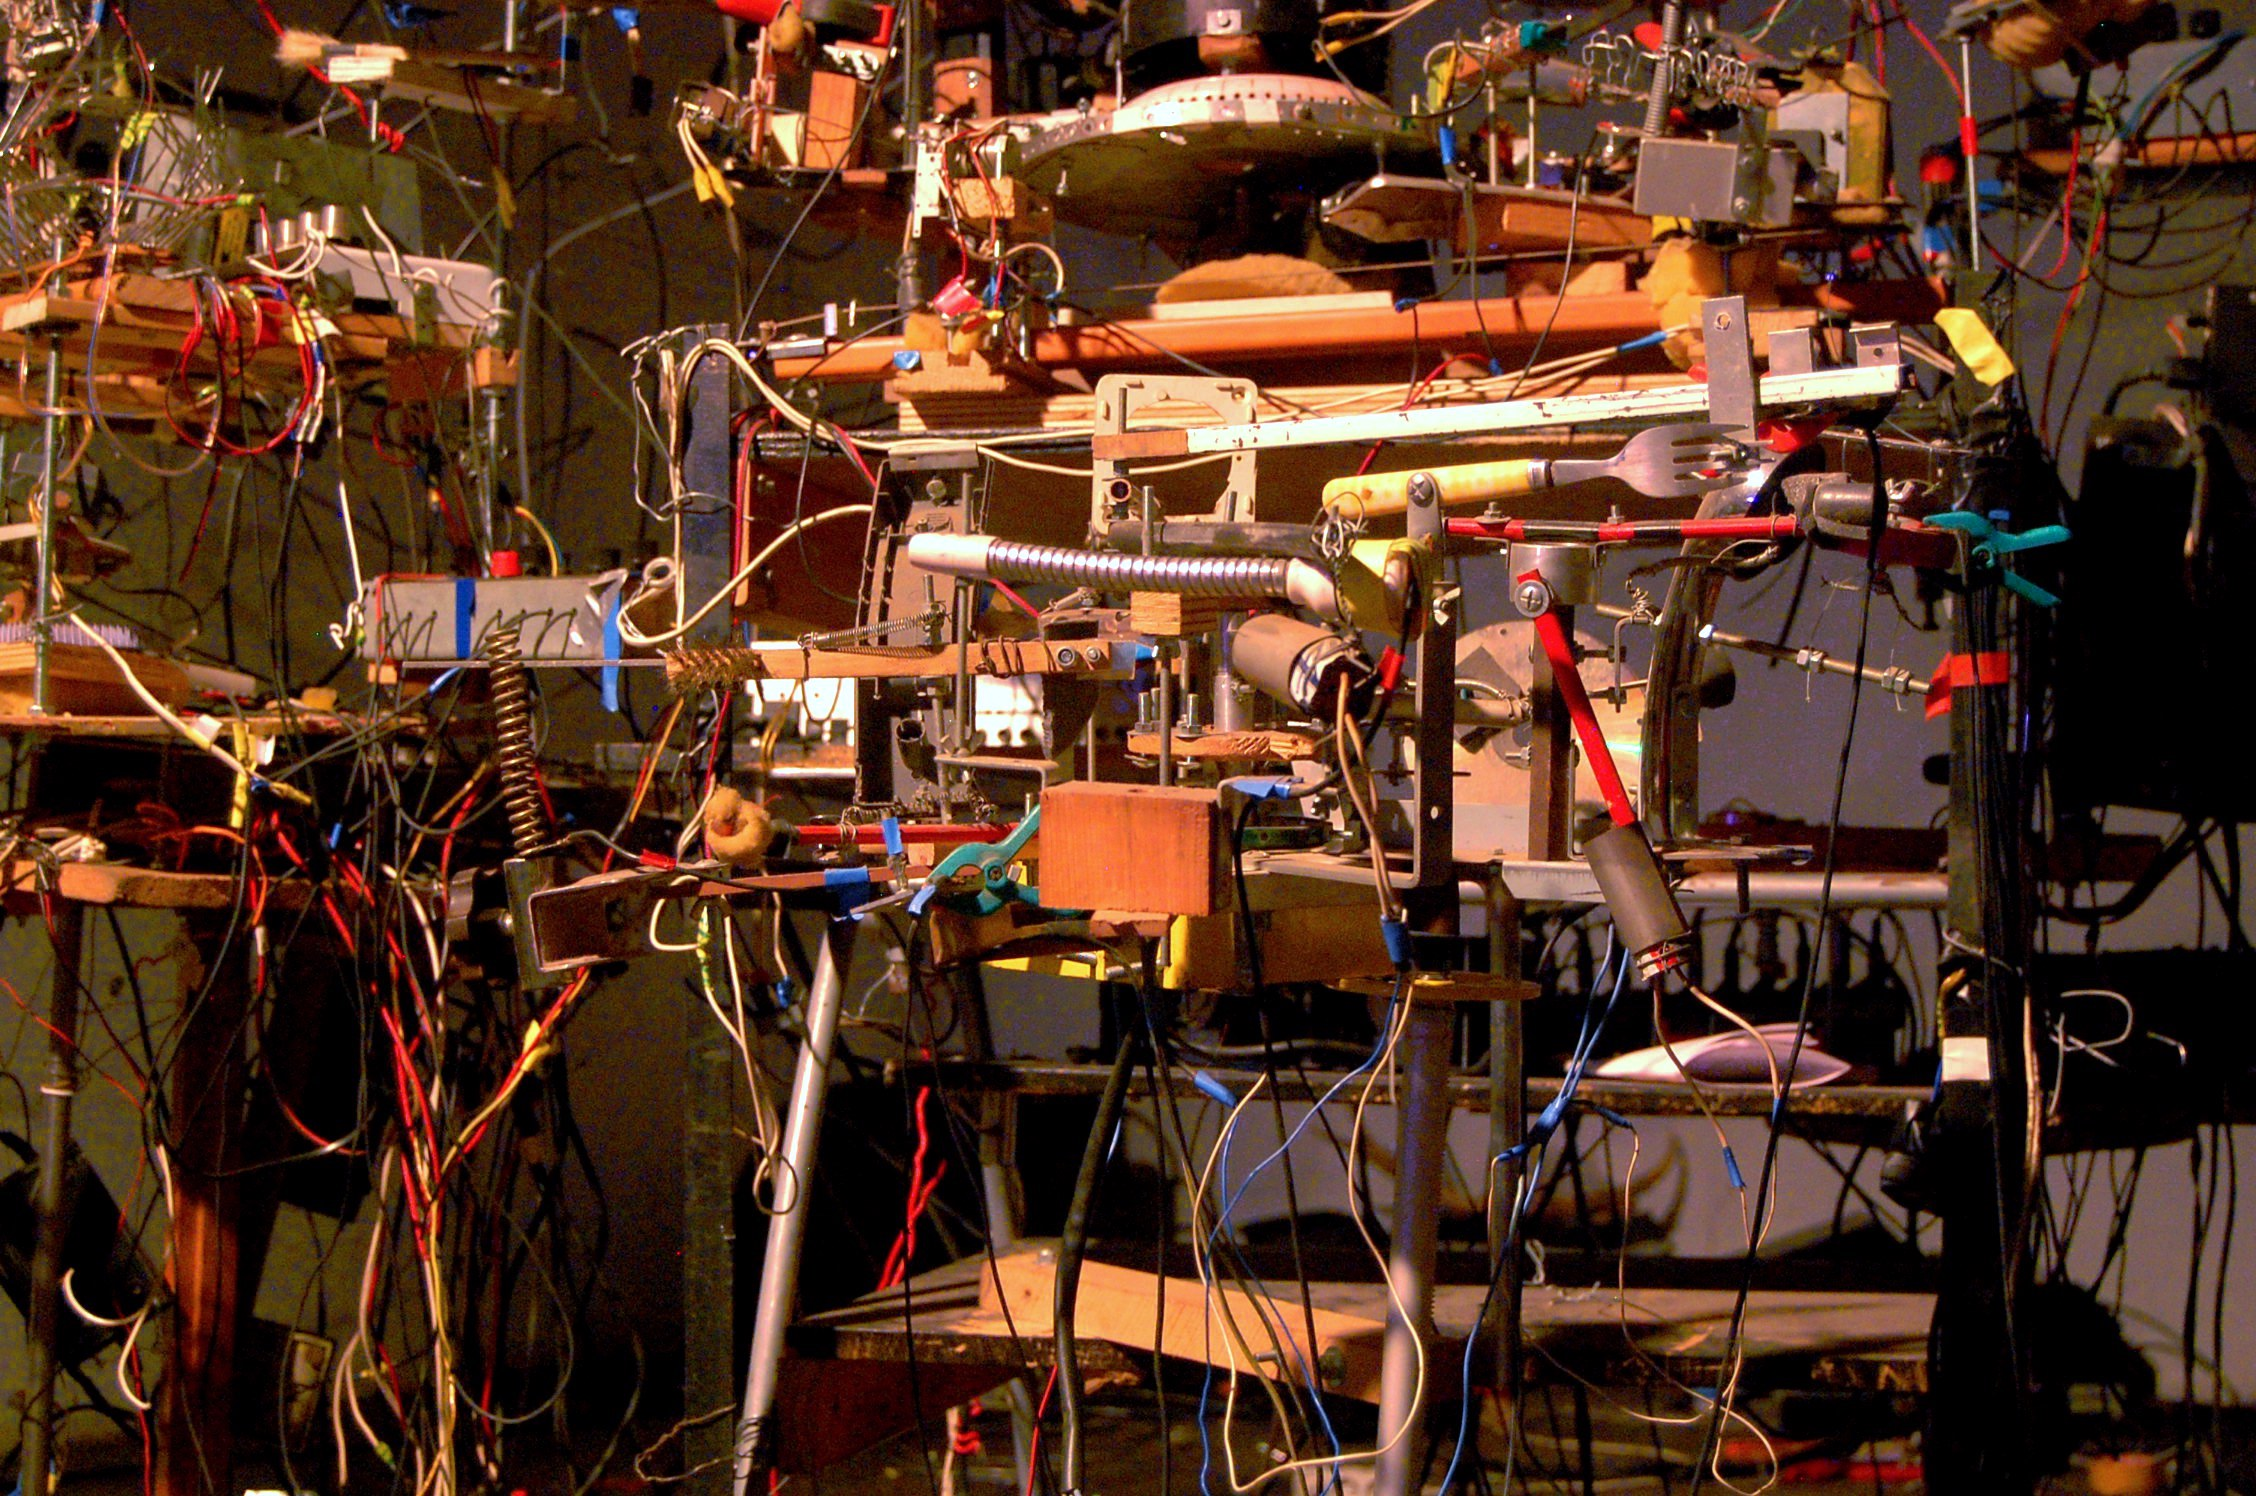
\includegraphics[width=\textwidth]{gfx/02_ephemeral/PierreGordeff.jpg}
	\caption{Détail d'un instrument de Pierre Gordeff.}
	\label{fig:ephemeral:Gordeff}
\end{figure}

\subsection{Cuisiner des instruments à la volée}

\noindent Une autre raison qui contribue à la stabilité des instruments acoustiques est liée à leur physicalité et à leur fabrication, qui demande un travail considérable en regard de l'arrangement virtuel de blocs logiciels - il faut plus de deux mois pour construire un violoncelle pour un luthier qui connaît son métier ! A l'inverse, John Bowers et al. ont promu l'utilisation d'objets prêts à l'emploi comme ``infra-instruments'' semi-fabriqués \cite{bowers_not_2005} et comme instruments ``pin-and-play'' \textit{ad hoc} \cite{bowers_creating_2006}, en repensant le cycle de vie d'un instrument avec ce type de montage éphémère et rapidement assemblé.\\
\indent Plus généralement, lorsqu'on crée un \gls{DMI} avec un environnement de programmation audio, le logiciel fournit non seulement des fonctions de base mais aussi des bibliothèques, des exemples prêts à l'emploi, complétés par d'innombrables ressources en ligne, prêtes à être téléchargées, copiées et collées.\\
\indent Cela signifie que la conception d'un \gls{DMI} peut se faire très rapidement, de manière soustractive : plutôt que de partir d'une page blanche, il est possible de chercher une version proche de ce que l'on veut réaliser et de la modifier en partant de là. Nicolas Collins a comparé cette simplicité à la cuisine, en mettant l'accent sur sa démocratisation : \iquote{Ce que ça veut dire, c'est que si tu joues en live, si tu as vraiment besoin d'instruments spécialisés, cela s'apparente presque plus à de la cuisine qu'à de la fabrication d'instruments de musique. Tout le monde cuisine, tu n'as pas besoin d'aller dans une école pour chefs !} [Collins, communication personnelle, cf. \ref{appendix:collins}]\\
\indent Les évolutions récentes des langages de programmation audio tendent à aborder la question de la durabilité en créant des langages spécifiques à un domaine qui peuvent être exportés vers différentes pleteformes cibles. Les plates-formes hardware comme Bela ou The Owl\footnote{Bela: \url{https://bela.io}; The Owl: \url{https://www.rebeltech.org}} et les langages comme \gls{FAUST} développé par le \gls{GRAME} \cite{orlarey_faust_2008} ou SOUL annoncé par Roli\footnote{Announced at the Audio Developer Conference 2018. \url{https://youtu.be/-GhleKNaPdk}} reflètent tous cette tendance. Il est intéressant de noter que \gls{FAUST}, qui a été conçu dans une optique de préservation, facilite en même temps la conception d'instances éphémères en offrant à la fois un compilateur en ligne et une compilation à la volée\footnote{En s'appuyant sur l'infrastructure \gls{LLVM}}.
	
\subsection{Une relation tri-partite : répertoire / musicien / contexte}

\noindent Si nous cessons donc de considérer l'éphémèrité des instruments seulement comme un problème, nous pouvons envisager la manière dont longévité et éphémèrité peuvent s'articuler dans l'agentivité des pratiques liées aux \glspl{DMI}. Celles-ci peuvent être envisagées comme un couplage tripartite entre un ensemble de matériaux, un musicien et un contexte, chacun des membres présentant un degré différent de stabilité.

\subsubsection{Le grand répertoire}

\noindent Les composants d'un \gls{DMI} peuvent être considérés comme appartenant à un large répertoire patrimonial matériel et immatériel. Ce répertoire comprend notamment tous les matériaux physiques qui peuvent être utilisés dans la construction d'instruments acoustiques : matières premières, pièces usinées ou mécaniques. \\
\indent Le répertoire immatériel est l'ensemble des connaissances théoriques et du patrimoine culturel sur lesquels on peut s'appuyer lors de la fabrication d'un instrument\footnote{Bien évidemment, la connaissance pratique est aussi essentielle à la fabrication d'un instrument, même si elle n'appartient pas vraiment au patrimoine commun auquel je fais référence ici.} : théorie musicale, connaissances scientifiques et techniques, techniques de jeu établies, répertoire musical, etc. Cette connaissance oriente le façonnement les matériaux et guide leurs positionnements relatifs :  placement des frettes, accord des cordes, la disposition des touches, etc.\\
\indent Dans le cas des \gls{DMI}, cependant, le répertoire des matériaux physiques est considérablement élargi par des connaissances réifiées disponibles sous forme de matériaux numériques, soit sous forme de code informatique, soit sous forme d'ensembles de données (e.g. échantillons audio, réponses impulsionnelles, séquences de notes, etc.) qui permettent de façonner l'indentité et les qualités musicales d'un instrument au-delà de ce qui est possible avec les matériaux physiques.
Cet ensemble, aussi hétérogène qu'il puisse paraître, constitue un répertoire partageable dans lequel les luthiers numériques peuvent puiser les ingrédients nécessaires à la conception de leur instrument.

\subsubsection{Le musicien in-progress/in-process}

\noindent Le deuxième élément de l'agencement est le musicien\footnote{Ici, le terme générique de "musicien" représente principalement l'instrumentiste, mais comme rappelé précédemment, les frontières entre les rôles de d'instrumentiste, de compositeur et de luthier sont poreuses.}. Les musiciens sont vivants et sujets au changement : leurs connaissances, leur expérience et leurs désirs, leurs compétences et leur conscience musicale, leurs projets et leurs capacités physiques évoluent tout au long de leur existence. Cette évolution se reflète dans le dispositif instrumental, par l'ajout ou le retrait de composants, ou par le développement de nouveaux instruments liés à un nouveau projet musical. Ainsi, de la même manière qu'on peut apprendre à conduire un vélo à l'aide de roues latérales et de les enlever plus tard, les \glspl{DMI} se prêtent à une assistance évolutive pour un apprentissage progressif. Cette relation co-dynamique avec l'instrument peut aider à améliorer l'intimité\footnote{Sur la question du rapport d'intimité entre le musicien et un nouvel instrument, voir notamment les articles de Sydney Fels, e.g. \cite{fels_designing_2004}} entre le musicien et l'objet technique qui devient instrument.\\

\subsubsection{Le \textit{hic et nunc} de la performance}

\noindent Enfin, le \gls{DMI} peut être adapté au contexte de la performance, qui est généralement plus éphémère que les deux aspects mentionnés ci-dessus.
En composant son propre répertoire musical à partir du grand répertoire susmentionné et de sa propre expérience, le musicien sélectionne un sous-ensemble d'éléments dans la perspective d'une performance particulière, pour une proposition artistique singulière, et pour s'adapter aux conditions spatiales et temporelles de la performance, ainsi qu'au public. A titre d'exemple, le code qui se duplique sans peine offre des possibilités de redimensionner un \gls{DMI} soliste en instrument collectif, en distribuant le contrôle sur plusieurs interfaces. De nouveaux projets peuvent impliquer de repartir de zéro, mais les projets existants n'impliquent souvent que des ajustements contextuels plutôt qu'une reprogrammation complète de son propre système. Chris Kiefer et Thor Magnusson ont proposé le terme de ``pre-gramming'' \cite{kiefer_live_2019} pour décrire ce type particulier de préparation\footnote{dans le contexte du live-coding qui est le leur, Kiefer et Magnusson détournent en fait le terme ``pro-gramming'' pour désigner l'action de coder en live, face à un public, tandis que le ``pre-gramming'' est l'activité de programmation préalable à la ``pro-grammation''}.
	

\section{Jouer d'un DMI éphémère}

\noindent Comme nous pouvons le voir, la création d'un \gls{DMI} peut être un processus très rapide, consistant en l'assemblage d'éléments déjà pré-construits. Mais une fois l'assemblage terminé, comment apprendre à en jouer ?

\subsection{Composition, conception, apprentissage et jeu en parallèle}

\noindent Les instruments acoustiques traditionnels sont soutenus par des méthodes et un répertoire qui peuvent à leur tour s'appuyer sur la stabilité de l'instrument. Mais pour un nouveau \gls{DMI}, possiblement unique, possiblement éphémère, de telles ressources ne sont guère disponibles. Les logiciels sont au mieux livrés avec des manuels, mais ceux-ci expliquent généralement comment faire fonctionner le logiciel, pas comment jouer de la musique avec.\\
\indent De là, le processus d'apprentissage peut suivre deux directions apparemment opposées : trouver les bons gestes pour jouer les sons désirés et trouver les bons sons pour les gestes choisis. En conséquence, l'apprentissage d'un nouveau \gls{DMI} commence souvent dès sa conception et est un processus co-dynamique qui accompagne son développement jusqu'à la \textit{pré-grammation} de l'instrument, avec des allers-retours entre les moments de jeu et les moments de réglage.

\subsection{Entrer dans l'avenir à reculons}

\noindent Les \glspl{DMI} et leurs pratiques héritent du savoir-faire des musiques électroacoustiques thésaurisé depuis le milieu du XXème siècle. La pédagogie de la musique électroacoustique s'est essentiellement appuyée sur les théories musicales de l'écoute \cite{schaeffer_traite_1966} et des métaphores pour composer \cite{bayle_musique_1993}. Mais celles-ci furent conçues à une époque où la musique électroacoustique ne pouvait qu'être composée sur support, avant que les pratiques audio en temps réel ne permettent leur performance en live. En conséquence, ces théories étaient plus orientées vers la composition musicale que vers l'interprétation en tant que telle.
\indent En l'absence d'une notation musicale établie pour le son, la performance électronique expérimentale s'est en partie orientée vers l'improvisation libre, qui implique un lâcher prise permettant à l'instrument d'exprimer ses potentialités et une pratique de l'"auralité"\footnote{Décrite par Alain Savouret comme une théorie musicale pour l'audible.} pour ``entrer dans l'avenir à reculons'' \cite{savouret_introduction_2010} et réagir à ce qui sort de l'instrument plutôt que le maîtriser complètement.

\subsection{Trouver les résonances}

\noindent L'apprentissage d'un instrument (au-delà de l'apprentissage des idiomes établis pour cet instrument) nécessite donc une recherche de résonance. On peut faire l'expérience de cette résonance à un niveau acoustique, mais plus généralement comme une résonance empathique, qui consiste à s'immerger dans l'instrument pour trouver les espaces qui vont (re)sonner de manière satisfaisante, pour trouver les \textit{sweet spots}\footnote{Il n'existe pas de véritable équivalent français pour cette expression anglaise, désignant un équilibre optimal, un réglage bien ajusté, une zone idéale. Les ingénieurs du son l'utilisent notamment pour désigner l'emplacement d'écoute idéale par rapport à la position des haut-parleurs.} où ce que nous entendons rencontre ce que nous cherchions, parfois sans le savoir. La linéarité mathématique étant rarement satisfaisante au niveau perceptuel, cette exploration impliquant la coordination entre le jeu et l'écoute critique est essentielle pour ajuster les fonctions de transfert qui vont définir le comportement de l'instrument.

\subsection{Entomologie musicale (bestiaire)}

\noindent L'exploration musicale d'un \gls{DMI} fait surgir des formes musicales inconnues, comme des papillons éphémères. L'apprentissage d'un \gls{DMI} implique donc souvent une tâche similaire à celle de l'entomologiste, qui consiste à épingler ces créatures sonores et à leur donner un nom. Ce nommage permettra d'y revenir plus tard (en les sauvegardant dans des presets par exemple) ainsi que de discuter avec d'autres musiciens d'une performance qui, en l'absence d'idiomes musicaux établis sur lesquels s'appuyer, comme les gammes ou la signature temporelle, peut cruellement manquer de références. Une telle tâche a été menée dans le développement de ``John, le semi-conducteur'', un système de partition ouvert décrit dans \cite{goudard_john_2018} et dans le chapitre \ref{ch:notation}.\\
\todo{fusionner avec la section \ref{sec:ephemeral:vessels}?}


%-------------------------- Figure : Entomologie ----------------------------------
\begin{figure}[!htbp]
	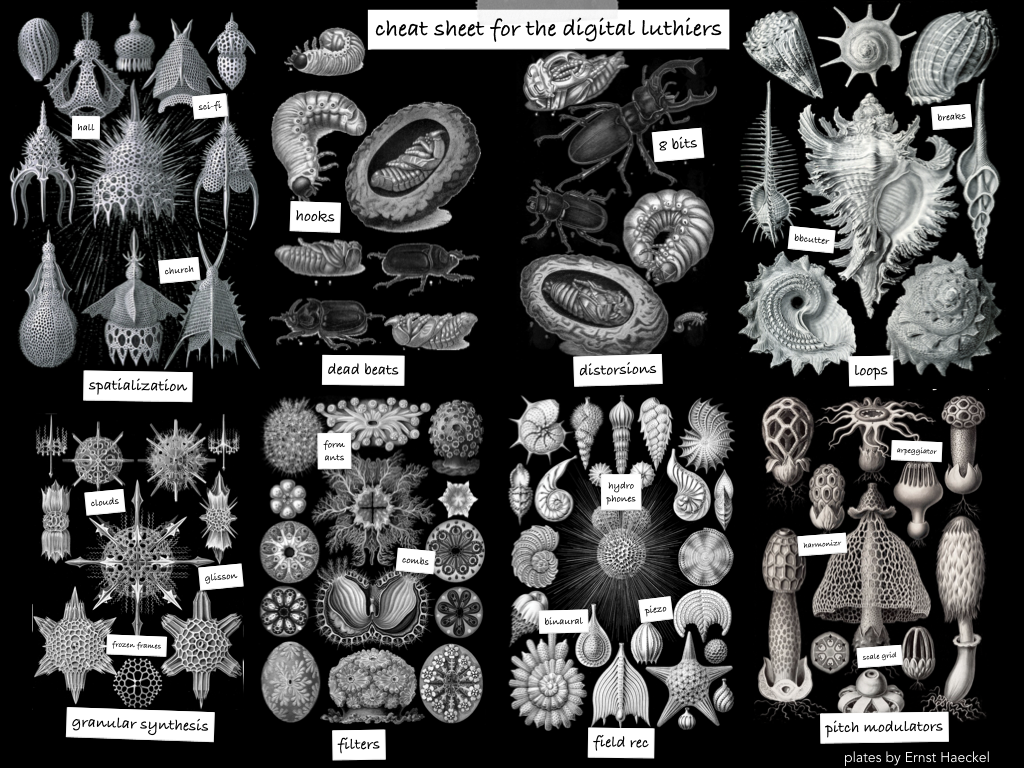
\includegraphics[width=\textwidth]{gfx/02_ephemeral/Bestiaire.png}
	\caption{Entomologie musicale}
	\label{fig:ephemeral:entomologie}
\end{figure}

\subsection{Pratique modulaire de la stabilité}

\noindent Si l'agencement éphémère d'un \gls{DMI} peut sembler trop instable pour pouvoir établir des méthodes pédagogiques pérennes, ses composantes individuelles peuvent offir des points d'accroche plus stables. Par exemple, si la performance est basée sur une partition écrite, l'instrumentiste peut apprendre l'enchaînement des gestes appropriés nécessaires à sa réalisation \footnote{La pièce ``Aphasia'' de Mark Applebaum (https://youtu.be/wWt1qh67EnA), où la performance repose sur des gestes et une bande sonore totalement notés, en est un exemple radical de ce point de vue là.}.\\
\indent En ce qui concerne le comportement du \gls{DMI}, on peut en partie transférer sa connaissance d'autres \glspl{DMI} à une nouvelle instance qu'on essaie d'apprendre. Par exemple, l'intégration d'une synthèse \gls{FM} dans un \gls{DMI} peut aider une personne familière avec ce type de synthèse à naviguer dans son espace timbral. Elle y retrouvera l'espace sonore caractéristique de la \gls{FM}\footnote{J'entend par là non seulement les différents timbres (cloches, sirènes, cuivres, etc.) caractéristique de cette synthèse, mais également la topologie de leur répartition dans l'espace paramétrique}, indépendamment de l'interface de contrôle qui y est branchée, en s'appuyant sur ses propres connaissances et représentations de l'espace de paramètres de la synthèse \gls{FM}. L'espace de timbre de diverses synthèses audio peut également être redistribué sur un espace perceptif commun et plus stable (en s'appuyant par exemple sur des paramètres perceptifs tels que la hauteur, le volume, la brillance, etc.) qui dissocie leur contrôle des différents espaces de paramètres respectifs, tels que présentés dans \cite{wessel_timbre_1979}, \cite{arfib_strategies_2002}, \cite{schwarz_sound_2012} ou \cite{tubb_divergent_2014}.\\

\indent De manière similaire, une expertise peut être acquise sur une interface gestuelle, qui invite à des gestes et des déplacements spécifiques \footnote{Par exemple, la scène "launchpad" s'est développée autour d'une interface particulière, le launchpad de Novation, qui doit en partie son succès à son prix abordable et sa simplicité d'usage (absence de vélocité \gls{MIDI}, une seule prise \gls{USB}, connection immédiate à Ableton Live). Les affrontements de virtuosité rythmique et la possibilité de programmer dynamiquement les couleurs (et le mapping) du launchpad en a fait un phénomène internet, à travers la publication de video de remix et de mashups virtoses sur YouTube. L'émergence de cette scène a donné lieu à un certain nombre de tutoriels vidéos pour apprendre à jouer, ainsi qu'à des logiciels pédagogiques dédiés (e.g. Melodics, ``a desktop app that teaches you to play MIDI keyboards, pad controllers, and MIDI drum kits.'' \url{https://melodics.com/})} ; cette expertise repose sur une mémoire spatiale incorporée, qui reste en partie indépendante des synthèses ou effets audio contrôlés par l'interface. La stabilité comportementale de l'instrument peut également être de nature virtuelle, par exemple en utilisant des modèles intermédiaires dynamiques \cite{goudard_dynamic_2011} (cf. \ref{sec:algorithms:MID}), qui peuvent servir de référence stable entre diverses synthèses et interfaces en évolution.
\noindent Dans l'ensemble, cette connaissance transposée et ``modulaire'' ne peut fournir que les grandes lignes de ce qui est nécessaire à la pratique subtile d'un instrument. Le diable se cache évidemment dans les détails.


\subsection{Les DMI comme vaisseau pour la mémoire}
\label{sec:ephemeral:vessels}

\noindent Les \glspl{DMI} s'apparentent ainsi à des vaisseaux hétérogènes, chargés de souvenirs de nos expériences d'interprétation, de composition ou de fabrication d'instruments. Les sons que nous recueillons, les algorithmes de synthèse que nous développons (ou téléchargeons), les paramètres que nous ajustons, les recettes de cuisine et les fonctions de transfert que nous élaborons avec soin, contribuent à l'évolution d'un répertoire personnel où se cristallisent des instances éphémères. Thor Magnusson a proposé le terme ``d'outil épistémique'' pour décrire le \glspl{DMI} comme \iquote{un outil conçu avec un tel degré de pertinence symbolique qu'il devient un système de connaissance et de pensée dans ses propres termes} \cite{magnusson_epistemic_2009}.\\
\indent Ainsi, les \glspl{DMI} se présentent comme des assemblages évolutifs de ces matériaux enregistrés et impliquent souvent des activités qui ne sont généralement pas associées à la pratique instrumentale, comme la gestion de fichiers, le versionnage du code, le recensement de ressources en ligne ou l'organisation de banques de sons, afin de pouvoir réunir ces ressources aussi rapidement que possible pour la performance.\\
\indent Il est remarquable que les possibilités de duplication et de diffusion offertes par les médias numériques et Internet n'aient pas conduit à la standardisation des instruments ; les instruments de musique numériques sont souvent très personnels et singuliers.

\section{Conclusion}

\noindent Ce chapitre a permi de présenter les \gls{DMI} à travers la notion d'assemblage éphémère qui les caractérise, en la considérant non pas seulement comme un problème, mais comme une modalité intrinsèque de leur ontologie. Au contraire d'exclure leur longévité, elle éclaire en fait la conception technique des environnements propices à leur développement et à leur durabilité.\\
\indent  L'éphémèrité des outils n'empêche pas la production de musique passionantes, ni la réalisation de performances musicales captivantes. Au contraire, elle peut à la fois aider à adapter les assemblages musicaux à des contextes essentiellement éphémères et défier la capacité de l'être humain à répondre à une dispositif musical fugace et indompté. En fin de compte, les grandes œuvres musicales semblent trouver leur chemin, soutenues par le soin et le travail de ceux qui reconnaissent ces œuvres comme des chefs-d'œuvre. Ces œuvres peuvent résister à l'épreuve du temps en étant dispersées, distribuées, transformées, recomposées, réinterprétées ou même renommées, par tous ceux qui y attachent de l'importance. Ce soin attentionné, mû par notre désir de musique, appartient probablement à la partie de notre mémoire que nous ne pouvons pas externaliser dans un outil et qui redéfinit la tradition et la préservation en dehors du cadre technologique.\\
\indent Dans le sable évoqué par Michel Chion, nous pouvons voir une autre métaphore intéressante pour les instruments de musique numériques, car dans une vie antérieure, le sable était une roche qui s'était atomisée, fragmentée en petits morceaux. La même chose semble s'être produite pour les instruments de musique, qui ont été atomisés en petits modules. Nous pouvons jouer avec le sable comme un matériau fluide, ou lui ajouter de l'eau, voire du ciment, pour lui donner une forme concrète.
\indent Si les technologies numériques arrivent un jour à maturité, nous pourrons peut-être compter sur des instruments numériques stables et durables. Dans ce cas, et faisant suite à la prémonition de Garsault, il ne faudra pas oublier de classer tous les instruments éphémères qui les ont précédés dans la catégorie des \iquote{instruments hors d'usage, mais qui peuvent revenir}.


\section{extra material}

Thor Magnusson in Sonic Writing (p12) : Anyone who plays a musical instrument will be familiar with the special moment when a new instrument is picked and its ergodynamics studied through play. (footnote : we often change our instruments during performance : we retune string instruments, change effect settings in electronics, and the \textit{whole point} of live coding is to create and redefine the instrument during play). This experience of ergodynamics recognises that an instrument is an object that never rests, or enter a period of stasis: that every time we pick it up there are new things to discover, new patterns our fingers know, because we have changed, the instrument has changed, and so has the whole world itself — the general performance context.

Risset dans \cite{genevois_les_1999} : ``La disponibilité `'d'accès'' gestuels tout à fait différents de accès instrumentaux risque de rester lettre morte, dans la mesure où il est improbable que des interprètes réalisent l'investissement considérable que représente l'apprenttissage d'un instrument complètement nouveaux s'ils n'ont pas l'assurance que cet instrument va durer et qu'un répertoire va se développer pour lui''

